\chapter{Black Holes, White Holes, and the Global Causal Diagram}

\lectureoverview{A horizon is locally ordinary and globally decisive. We begin with the near-horizon Schwarzschild metric, follow it outward with the Euclidean cigar analogy, and then ask what Alice and Bob can actually see. The singularity and the time-reversed white-hole region enlarge that local picture into the eternal Schwarzschild spacetime. Penrose compactification makes the causal structure finite and readable. The final step turns from an eternal solution to a black hole made by collapse, where Newton's shell theorem and Birkhoff's theorem supply the pieces to be joined.}

\section{From the Horizon to Infinity}

Near a sufficiently large Schwarzschild horizon, curvature is weak over a small laboratory and the radial-time geometry is approximately flat. The convenient radial variable is not the Schwarzschild coordinate \(r\), but the proper distance \(\rho\) measured outward from the horizon along a constant-time spatial slice:
\begin{equation}
\rho=0 \quad\Longleftrightarrow\quad r=2GM .
\label{eq:l04-rho-horizon}
\end{equation}
The convenient time coordinate is the dimensionless quantity
\begin{equation}
\omega=\frac{t}{4GM},
\label{eq:l04-omega}
\end{equation}
where \(c=1\). Thus \(\omega\) is Schwarzschild time measured in units of twice the Schwarzschild radius.

With the mostly-plus convention, the near-horizon radial-time metric is
\begin{equation}
ds^2\approx-\rho^2d\omega^2+d\rho^2.
\label{eq:l04-rindler}
\end{equation}
The angular two-sphere has been suppressed because the present argument concerns only time and radial distance.

\begin{figure}[htbp]
\centering

\includegraphics[width=0.72\textwidth]{lecture_04_figure_02.png}
\caption{The near-horizon metric and the rescaled Schwarzschild time.}
\lectureframe{00:05:46.800}
\end{figure}

Equation~\eqref{eq:l04-rindler} has the same relation to Minkowski spacetime that polar coordinates have to a Euclidean plane. For
\begin{equation}
T=\rho\sinh\omega,
\qquad
X=\rho\cosh\omega,
\end{equation}
one obtains
\begin{equation}
-dT^2+dX^2=-\rho^2d\omega^2+d\rho^2.
\end{equation}
Lines of constant \(\rho\) are hyperbolae \(X^2-T^2=\rho^2\), while \(\omega\) runs from the remote past to the remote future. The two null lines \(X=\pm T\) meet at the bifurcation point of the reduced diagram. In four dimensions that point represents a two-sphere, and the future and past null sheets form a bifurcate Killing horizon.\editorialnote{Calling only the crossing point the bifurcate horizon is useful shorthand in the radial diagram. More precisely, the two horizon branches intersect on a bifurcation two-sphere.}

\subsection{The far region}

The radial-time part of the Schwarzschild metric is
\begin{equation}
ds^2
=-\left(1-\frac{2GM}{r}\right)dt^2
+\frac{dr^2}{1-\frac{2GM}{r}}.
\label{eq:l04-schwarzschild}
\end{equation}
Far from the hole, \(r\gg2GM\), the metric approaches
\begin{equation}
ds^2\approx-dt^2+dr^2.
\end{equation}
There \(r\) and \(\rho\) differ only by an inessential additive correction, so with \(dt=4GM\,d\omega\),
\begin{equation}
ds^2\approx-(4GM)^2d\omega^2+d\rho^2.
\label{eq:l04-far}
\end{equation}
The radial coefficient is simple in both limits. The time coefficient is what changes:
\begin{equation}
ds^2\approx
\begin{cases}
-\rho^2d\omega^2+d\rho^2, & \rho\ll GM,\\[3pt]
-(4GM)^2d\omega^2+d\rho^2, & \rho\gg GM.
\end{cases}
\label{eq:l04-two-limits}
\end{equation}
Along a hovering trajectory, \(d\rho=0\). Close to the horizon,
\begin{equation}
d\tau=\rho\,d\omega,
\end{equation}
whereas far away \(d\tau\approx4GM\,d\omega=dt\). For a fixed increment of the exterior time coordinate, less and less proper time elapses on a clock held closer to the horizon.

\subsection{The cigar}

Spacetime is difficult to picture, so replace the timelike direction by an ordinary angular direction. Write
\begin{equation}
d\ell^2=F(\rho)^2d\theta^2+d\rho^2,
\qquad
F(\rho)\sim
\begin{cases}
\rho, & \rho\to0,\\
4GM, & \rho\to\infty.
\end{cases}
\label{eq:l04-cigar}
\end{equation}
Near \(\rho=0\), this is the plane in polar coordinates. Far away, the circumference no longer grows with radius:
\begin{equation}
C_\infty=\int_0^{2\pi}4GM\,d\theta=8\pi GM.
\label{eq:l04-cigar-circumference}
\end{equation}
The surface therefore rounds off at one end and approaches a cylinder at the other. It looks like a cigar.

\begin{figure}[htbp]
\centering

\includegraphics[width=0.74\textwidth]{lecture_04_figure_03.png}
\caption{The Euclidean comparison: a polar tip joined to an asymptotic cylinder of circumference \(8\pi GM\).}
\lectureframe{00:14:05.000}
\end{figure}

The larger the mass, the larger the asymptotic girth and the gentler the bend near the tip. A small hole corresponds to a tightly curved cigar; a large hole has a broad, weakly curved tip. This is a picture of the interpolation in Equation~\eqref{eq:l04-two-limits}, not an embedding of the Lorentzian black hole itself.\editorialnote{The precise geometric object is obtained by continuing Schwarzschild time to imaginary time. Smoothness at the tip then fixes the Euclidean-time period to \(8\pi GM\), the same scale that later determines the Hawking temperature. The lecture uses only the visual analogy here.}

\section{Reading the Horizon Causally}

Outside the hole, \(\rho>0\), a stationary observer follows a constant-\(\rho\) hyperbola. Far away, only modest acceleration is needed to resist gravity; close to the horizon, the required proper acceleration grows without bound. Once a worldline crosses the future null boundary, no future-directed causal signal from it can reach the exterior.

\begin{classroomqa}
\audiencequestion{Are light rays straight lines on this diagram?\lecturetimestamp{00:20:21}}
\lecturerresponse{Radial light rays are drawn at \(45^\circ\), unless a different convention is stated. An ingoing ray crosses the horizon; an outgoing ray that is already inside cannot cross back to the exterior.}
\end{classroomqa}

\begin{classroomqa}
\audiencequestion{Does an ingoing light ray stay on the horizon?\lecturetimestamp{00:21:12}}
\lecturerresponse{No. A ray aimed inward crosses the future horizon and continues into the black-hole interior. Only a horizon generator itself remains on the null boundary.}
\end{classroomqa}

\subsection{Bob watches Alice}

Let Bob hover outside at fixed radius while Alice falls inward. Bob sees Alice only by receiving outward-going light from her. Suppose she waves periodically according to her own clock. Signals emitted later in her fall take progressively longer Schwarzschild times to reach Bob, and he receives fewer waves per unit time. No signal emitted after horizon crossing can return to him.

The Rindler coordinates expose the limiting behavior. Define the outgoing null coordinate
\begin{equation}
U=T-X=-\rho e^{-\omega}.
\end{equation}
Approaching the future horizon means \(U\to0^{-}\), which requires \(\omega\to+\infty\) for fixed exterior \(\rho\). A finite crossing event for Alice is therefore pushed to infinite exterior time. Successive wave crests arrive with exponentially increasing separation, so their frequency is exponentially redshifted.\editorialnote{This null-coordinate calculation supplies the mathematical form of the redshift described qualitatively in the classroom. It uses only the local Rindler approximation.}

At first Bob receives optical light, then infrared, then radio waves of enormous wavelength. The useful statement is not that Alice remains as a permanently visible photograph on the horizon. She becomes dimmer, redder, and finally undetectable.

\begin{classroomqa}
\audiencequestion{Does Bob see Alice frozen at one exact place outside the horizon?\lecturetimestamp{00:26:31}}
\lecturerresponse{In the classical exterior-coordinate description, images received at later and later times come from events ever closer to the horizon. The limiting image is frozen there, but its radiation is redshifted until it effectively disappears. Quantum black-hole physics has not yet entered this account.}
\end{classroomqa}

\begin{classroomqa}
\audiencequestion{As Alice fades, does she also look compressed?\lecturetimestamp{00:28:34}}
\lecturerresponse{Yes. Relative motion produces longitudinal Lorentz contraction in the exterior description. The important observational effect here is still the redshift: her internal oscillations appear slower and the received wavelength grows.}
\end{classroomqa}

\subsection{Alice watches Bob}

Alice's proper time remains regular at the horizon. She continues to receive inward-going signals from Bob after crossing, because those signals follow the same causal direction as she does. She cannot reply to the exterior once she is inside. The horizon is one-way, not a wall encountered symmetrically from both sides.

\begin{classroomqa}
\audiencequestion{Does Alice see Bob's light blueshifted as she falls through?\lecturetimestamp{00:30:29}}
\lecturerresponse{In the picture being used, she sees Bob receding and his signals shifted toward the red; nothing singular occurs at her crossing. The precise frequency shift depends on both worldlines and on when Bob emits, so the invariant statement is that her measured frequency remains finite at a regular horizon.}
\end{classroomqa}

\begin{classroomqa}
\audiencequestion{Does the same causal restriction apply to gravitons?\lecturetimestamp{00:31:15}}
\lecturerresponse{It applies to genuine gravitational radiation just as it applies to photons. No radiative disturbance emitted from behind the future horizon can reach Bob.}
\end{classroomqa}

\begin{classroomqa}
\audiencequestion{When Alice falls in, does her energy increase the mass and radius of the hole?\lecturetimestamp{00:31:43}}
\lecturerresponse{Yes. Once her energy is included in the black hole, its mass rises and its Schwarzschild radius \(R_s=2GM\) rises with it. The dynamical formation problem will make that statement geometric.}
\end{classroomqa}

\subsection{Why the exterior still has gravity}

A black hole is dark but not gravity-free. A stationary gravitational field is not a stream of on-shell gravitons continually escaping from the interior. It is the already established exterior geometry. If the source changes, the change in the field propagates causally; a distant observer cannot detect that change before a light signal could arrive.

\begin{classroomqa}
\audiencequestion{If gravitons cannot escape, why does the black hole exert gravity at all?\lecturetimestamp{00:32:04}}
\lecturerresponse{The static field is already present outside. One may loosely describe it using virtual gravitons, but those are not detectable particles carrying fresh messages from the interior. What is limited by the speed of light is a change in the field, including gravitational radiation.}
\end{classroomqa}

\begin{classroomqa}
\audiencequestion{How can virtual gravitons be reconciled with the statement that a field change travels at light speed?\lecturetimestamp{00:34:02}}
\lecturerresponse{Virtual quanta are bookkeeping elements in a perturbative calculation, not signal-carrying particles with measurable trajectories. Gauge-invariant disturbances and information propagate causally. The same distinction appears between a static electromagnetic field and electromagnetic radiation.}
\end{classroomqa}

The classroom language that virtual gravitons can exceed the speed of light should therefore not be read as superluminal communication.\editorialnote{Off-shell virtual particles need not satisfy the on-shell dispersion relation, but they are not observables and cannot be used to transmit information. In general relativity the clean description is simpler: the stationary exterior metric exists, while changes of the gravitational field have causal propagation.}

\section{Can Alice Still See Her Feet?}

Let Alice fall feet first. Her feet cross the horizon before her head. When she looks down, she never sees the simultaneous event on the foot worldline; light takes time to travel, so she sees her feet at a slightly earlier event. There is a continuous sequence of such past events before and after her head crosses. Nothing locally discontinuous happens merely because one part of her body has passed \(r=2GM\).

The dangerous experiment is to reverse course after the feet are inside. To keep her head outside, Alice must accelerate outward. Her feet, already beyond the future horizon, cannot follow an exterior hovering trajectory. The separation in the accelerated frame grows without bound, and a material body cannot remain rigid across that causal boundary. She must either fall freely with her feet or be torn apart while attempting to hold the rest of herself outside.

This stretching is not a divergent tidal force at a large horizon. It is the consequence of demanding incompatible worldlines for an extended body.\editorialnote{A sufficiently large Schwarzschild horizon has small tidal curvature. The pathology in this thought experiment comes from the attempted acceleration and rigidity constraint, not from a local curvature singularity at the horizon.}

\section{The Singularity Is in the Future}

Return to Equation~\eqref{eq:l04-schwarzschild}. Outside,
\begin{equation}
1-\frac{2GM}{r}>0,
\end{equation}
so \(t\) is timelike and \(r\) is spacelike in Schwarzschild coordinates. Inside,
\begin{equation}
1-\frac{2GM}{r}<0,
\end{equation}
and those coordinate roles reverse: decreasing \(r\) is a timelike direction. This does not mean that space physically turns into time at the horizon. It means that the Schwarzschild chart degenerates there and that its labels have a different causal character inside.

The genuine singularity is at
\begin{equation}
r=0.
\end{equation}
It is not a vertical worldline representing a place one might avoid. It is a spacelike future boundary. Once Alice enters the black-hole region, every future-directed timelike or null path ends there. The curvature invariant
\begin{equation}
R_{\mu\nu\rho\sigma}R^{\mu\nu\rho\sigma}
=\frac{48G^2M^2}{r^6}
\label{eq:l04-kretschmann}
\end{equation}
diverges as \(r\to0\), whereas it is finite at \(r=2GM\).\editorialnote{Equation~\eqref{eq:l04-kretschmann} is the standard Schwarzschild Kretschmann scalar. It makes invariant the distinction drawn geometrically in the lecture between the regular horizon and the curvature singularity.}

\section{Time Reversal and the White Hole}

The Schwarzschild metric is independent of \(t\), and \(dt^2\) is unchanged by \(t\mapsto-t\). Its maximal extension is therefore symmetric under time reversal. Alongside the future singularity and future horizon, the mathematical solution contains a past singularity and a past horizon.

Time-reverse Alice's fall. She now emerges from the past singularity, crosses the past horizon outward, and appears in Bob's exterior. That region is called a white hole. It is not an escape route from the future black-hole interior: the future and past horizons are different null boundaries.

\begin{classroomqa}
\audiencequestion{If Alice cannot cross outward through the black-hole horizon, how can the reversed Alice come out?\lecturetimestamp{00:50:24}}
\lecturerresponse{She does not cross outward through the future horizon. She crosses outward through the past horizon, exactly as the time reverse of ordinary infall. The future black-hole region still has no outward causal path.}
\end{classroomqa}

\begin{classroomqa}
\audiencequestion{Must Bob's entire history also be run backward in the white-hole picture?\lecturetimestamp{00:52:15}}
\lecturerresponse{No. The extended geometry admits a history in which Bob remains in the exterior while Alice emerges from the past horizon. The puzzle is not mathematical consistency; it is the extraordinary initial condition represented by the past singularity.}
\end{classroomqa}

\begin{figure}[htbp]
\centering

\includegraphics[width=0.72\textwidth]{lecture_04_figure_04.png}
\caption{The developed causal sketch: crossed horizons, future and past singularity curves, and observer trajectories accumulated during the discussion.}
\lectureframe{01:00:19.818}
\end{figure}

\begin{figure}[htbp]
\centering
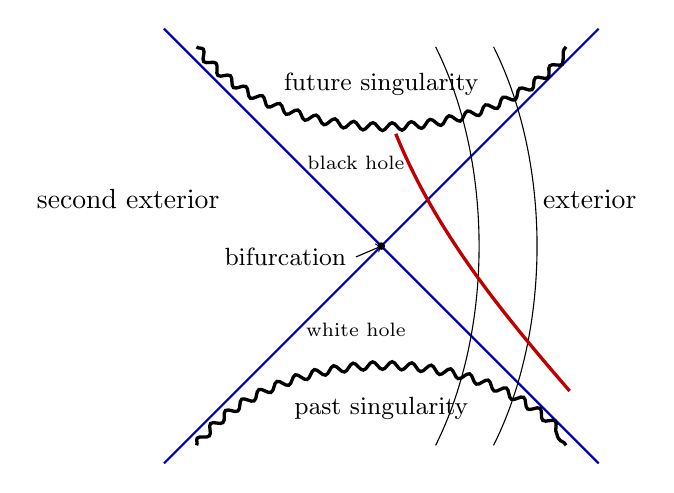
\begin{tikzpicture}[scale=0.92]
\draw[blue!75!black,thick] (-3,-3) -- (3,3);
\draw[blue!75!black,thick] (-3,3) -- (3,-3);
\draw[very thick,decorate,decoration={snake,amplitude=1.4pt,segment length=7pt}]
  (-2.55,2.75) .. controls (-1.45,1.35) and (1.45,1.35) .. (2.55,2.75);
\draw[very thick,decorate,decoration={snake,amplitude=1.4pt,segment length=7pt}]
  (-2.55,-2.75) .. controls (-1.45,-1.35) and (1.45,-1.35) .. (2.55,-2.75);
\draw (0.75,-2.75) .. controls (1.55,-1.15) and (1.55,1.15) .. (0.75,2.75);
\draw (1.55,-2.75) .. controls (2.35,-1.15) and (2.35,1.15) .. (1.55,2.75);
\draw[red!75!black,very thick] (2.6,-2.0) .. controls (1.65,-0.9) and (0.75,0.2) .. (0.2,1.55);
\fill (0,0) circle (1.5pt);
\node[above,font=\small] at (0,1.95) {future singularity};
\node[below,font=\small] at (0,-1.95) {past singularity};
\node[right] at (2.10,0.65) {exterior};
\node[left] at (-2.10,0.65) {second exterior};
\node[font=\scriptsize] at (-0.35,1.15) {black hole};
\node[font=\scriptsize] at (-0.35,-1.15) {white hole};
\node[font=\small,anchor=east] (bifurcation-label) at (-0.35,-0.15) {bifurcation};
\draw[->,thin] (bifurcation-label.east) -- (0,0);
\end{tikzpicture}
\caption{A cleaned uncompactified causal picture. Null horizons cross at the bifurcation surface; the spacelike singularities lie in the future and past wedges.}
\end{figure}

\subsection{Possible is not typical}

Microscopic mechanics is time-reversal invariant to an excellent approximation, yet macroscopic histories have a preferred direction. A bomb easily explodes; scattered fragments almost never reconvene to rebuild it. A ball easily rolls from an unstable summit; a randomly thrown ball almost never comes to rest precisely there. A racked triangle of billiard balls readily scatters, while scattered balls do not spontaneously arrange themselves into the rack. An ice cube melts in hot water, while the water almost never expels a newly assembled ice cube.

The distinction is entropy. A low-entropy macrostate occupies a tiny region of phase space; a high-entropy macrostate contains an enormous number of microscopic arrangements. The equations permit the reversed trajectory, but preparing its initial microstate requires fantastically precise correlations.

\begin{classroomqa}
\audiencequestion{Is not each exact scattered configuration just as unlikely as the exact time-reversed one?\lecturetimestamp{00:56:55}}
\lecturerresponse{Yes, for individually specified microstates. The asymmetry appears when we compare macrostates. A scattered arrangement includes vastly more microstates than a precisely assembled triangle, so almost every microscopic state compatible with the first description remains macroscopically disordered.}
\end{classroomqa}

A white hole that emits a fully organized Alice is the gravitational version of such an entropy-lowering history. It is allowed by the reversible equations but requires an extraordinarily special past. The horizon itself carries entropy and hidden microscopic information, so an Alice-sized fluctuation is not logically forbidden; it is overwhelmingly suppressed.

\begin{classroomqa}
\audiencequestion{Would such a fluctuation be quantum mechanical or thermal?\lecturetimestamp{00:59:48}}
\lecturerresponse{Both kinds can contribute. In an ordinary hot system the dominant language is thermal fluctuation; for a black hole, quantum and thermal effects are intertwined. Either way, the central suppression is entropic.}
\end{classroomqa}

\section{Proper Distance and Penrose Compactification}

Before drawing the global spacetime, we should make the radial jargon precise. Proper time is what a clock measures along a timelike worldline. Proper distance is what a chain of local meter sticks measures along a chosen spacelike curve. For the Schwarzschild constant-\(t\) slice,
\begin{equation}
d\rho=\frac{dr}{\sqrt{1-2GM/r}}.
\label{eq:l04-proper-distance}
\end{equation}
Thus \(r\) is an areal coordinate, not the direct meter-stick distance from the horizon.

Now begin with radial flat spacetime. Keep only \(t\) and \(\rho\ge0\). The line \(\rho=0\) is the spatial origin, and a radial light ray entering the origin continues outward on the opposite physical side, which appears as a reflection in the reduced half-plane.

A Penrose diagram maps all finite and infinite values of \(t\) and \(\rho\) into a finite region while preserving null directions. Its two rules are:
\begin{enumerate}
\item compactify the entire spacetime into a finite domain;
\item keep radial light rays at \(45^\circ\).
\end{enumerate}
Lengths and ordinary angles are distorted; causal relations are not.

\begin{figure}[htbp]
\centering

\includegraphics[width=0.70\textwidth]{lecture_04_figure_06.png}
\caption{The completed compactification grid for radial Minkowski spacetime. Infinite time lies at the upper and lower left endpoints, and infinite radius is compressed to the right tip.}
\lectureframe{01:14:44.040}
\end{figure}

\begin{figure}[htbp]
\centering
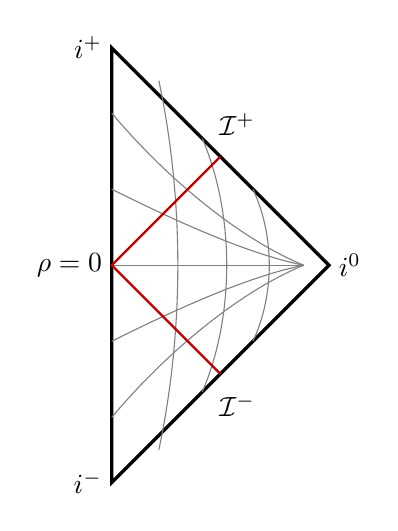
\begin{tikzpicture}[scale=0.92]
\coordinate (im) at (0,-3);
\coordinate (ip) at (0,3);
\coordinate (iz) at (3,0);
\draw[very thick] (im) -- (ip) -- (iz) -- cycle;
\draw[gray] (0,-2.1) .. controls (0.8,-1.15) and (1.8,-0.35) .. (2.65,0);
\draw[gray] (0,-1.05) .. controls (0.9,-0.6) and (1.9,-0.15) .. (2.65,0);
\draw[gray] (0,0) -- (2.65,0);
\draw[gray] (0,1.05) .. controls (0.9,0.6) and (1.9,0.15) .. (2.65,0);
\draw[gray] (0,2.1) .. controls (0.8,1.15) and (1.8,0.35) .. (2.65,0);
\draw[gray] (0.65,-2.55) .. controls (1.0,-0.9) and (1.0,0.9) .. (0.65,2.55);
\draw[gray] (1.25,-1.75) .. controls (1.7,-0.7) and (1.7,0.7) .. (1.25,1.75);
\draw[gray] (1.95,-1.05) .. controls (2.25,-0.4) and (2.25,0.4) .. (1.95,1.05);
\draw[red!75!black,thick] (1.5,-1.5) -- (0,0) -- (1.5,1.5);
\node[left] at (ip) {\(i^+\)};
\node[left] at (im) {\(i^-\)};
\node[right] at (iz) {\(i^0\)};
\node[above right] at (1.35,1.65) {\(\mathcal{I}^+\)};
\node[below right] at (1.35,-1.65) {\(\mathcal{I}^-\)};
\node[left] at (0,0) {\(\rho=0\)};
\end{tikzpicture}
\caption{Radial Minkowski spacetime in a finite triangle. The red null ray enters from \(\mathcal{I}^-\), reaches the origin, and leaves through \(\mathcal{I}^+\).}
\label{fig:l04-flat-penrose}
\end{figure}

The endpoints have distinct causal meanings:
\begin{align}
i^-&:\ \text{past timelike infinity},&
i^+&:\ \text{future timelike infinity},\\
i^0&:\ \text{spatial infinity},&
\mathcal{I}^-&:\ \text{past null infinity},&
\mathcal{I}^+&:\ \text{future null infinity}.
\end{align}
The script-\(I\) symbols \(\mathcal{I}^{\pm}\) are pronounced scri minus and scri plus.

\begin{classroomqa}
\audiencequestion{Should a null ray pass through the corners of every distorted grid cell, and therefore curve slightly?\lecturetimestamp{01:11:08}}
\lecturerresponse{If the full coordinate grid were drawn exactly, its intersections would be consistent with the null curve. The essential construction is conformal: radial null directions remain at \(45^\circ\), even though the constant-\(t\) and constant-\(\rho\) grid lines bend and crowd.}
\end{classroomqa}

\begin{classroomqa}
\audiencequestion{How is a light ray drawn if it misses the origin?\lecturetimestamp{01:11:45}}
\lecturerresponse{It reaches a nonzero distance of closest approach and returns outward. Once angular motion is retained, its projected radial path need not be a single straight \(45^\circ\) line.}
\end{classroomqa}

\begin{classroomqa}
\audiencequestion{Then why is that light ray not at \(45^\circ\)?\lecturetimestamp{01:12:49}}
\lecturerresponse{The \(45^\circ\) rule was stated for radial light rays. A null ray carrying angular momentum uses part of its motion in the angular directions, so its projection onto the \(t\)-\(\rho\) plane is not radial.}
\end{classroomqa}

\section{The Eternal Schwarzschild Diagram}

Compactifying the maximally extended Schwarzschild geometry produces four regions. The right and left diamonds are asymptotically flat exteriors. The upper triangle is the black-hole interior, bounded in the future by the spacelike singularity. The lower triangle is the white-hole region, bounded in the past by the past singularity.

\begin{figure}[htbp]
\centering

\includegraphics[width=0.74\textwidth]{lecture_04_figure_07.png}
\caption{The completed eternal Schwarzschild Penrose diagram, with singularities, horizons, null trajectories, and one asymptotic boundary marked on the board.}
\lectureframe{01:21:30.000}
\end{figure}

\begin{figure}[htbp]
\centering
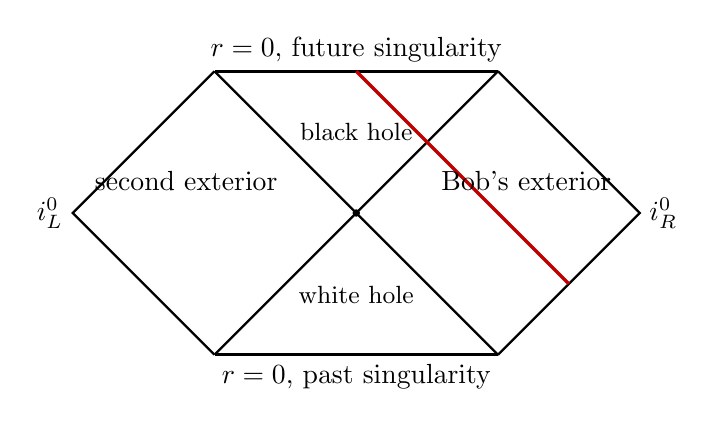
\begin{tikzpicture}[scale=0.90]
\coordinate (C) at (0,0);
\coordinate (TL) at (-2,2);
\coordinate (TR) at (2,2);
\coordinate (BL) at (-2,-2);
\coordinate (BR) at (2,-2);
\coordinate (L) at (-4.0,0);
\coordinate (R) at (4.0,0);
\draw[very thick] (TL) -- (TR);
\draw[very thick] (BL) -- (BR);
\draw[thick] (C) -- (TL) (C) -- (TR) (C) -- (BL) (C) -- (BR);
\draw[thick] (TL) -- (L) -- (BL);
\draw[thick] (TR) -- (R) -- (BR);
\draw[red!75!black,very thick] (3,-1) -- (1,1) -- (0,2);
\node[above] at (0,2) {\(r=0\), future singularity};
\node[below] at (0,-2) {\(r=0\), past singularity};
\node[font=\small] at (0,1.15) {black hole};
\node[font=\small] at (0,-1.15) {white hole};
\node at (2.4,0.45) {Bob's exterior};
\node at (-2.4,0.45) {second exterior};
\node[right] at (R) {\(i^0_R\)};
\node[left] at (L) {\(i^0_L\)};
\fill (C) circle (1.5pt);
\end{tikzpicture}
\caption{The four regions of eternal Schwarzschild. An ingoing radial light ray crosses the future horizon and terminates at \(r=0\).}
\label{fig:l04-eternal}
\end{figure}

An ingoing radial light ray from \(\mathcal{I}^-\) crosses the future horizon and ends on the singularity. Every causal curve in the upper triangle shares that fate. The second exterior is often described as the other mouth of an Einstein--Rosen bridge, but it is not traversable: any attempted causal trip from one exterior to the other enters the black-hole region and reaches the singularity.

\begin{classroomqa}
\audiencequestion{Are the two exterior worlds connected by a wormhole, and can one signal through it?\lecturetimestamp{01:22:21}}
\lecturerresponse{The eternal geometry contains an Einstein--Rosen bridge on suitable spatial slices, but no causal signal crosses from one exterior to the other. The bridge pinches off too quickly; even light entering a horizon ends at the future singularity.}
\end{classroomqa}

This diagram describes a hole that has existed for all time. Real astrophysical holes form from collapsing matter. Their causal diagram has no past white-hole singularity and no second asymptotic exterior. To construct that geometry, we need to understand spherical shells.

\section{Preparing a Black Hole by Collapse}

Imagine a diffuse spherical shell of incoming particles. They may be photons: energy gravitates, so a sufficiently concentrated pulse of radiation can form a black hole. Before collapse the central region resembles empty flat spacetime; after enough energy is compressed, the exterior resembles Schwarzschild. The task is to join those regions across the moving shell.

\subsection{Newton's shell theorem}

For a spherically symmetric Newtonian shell of total mass \(M\), Gauss's law for gravity reads
\begin{equation}
\oint \mathbf{g}\cdot d\mathbf{A}=-4\pi G M_{\mathrm{enc}}.
\label{eq:l04-gauss-gravity}
\end{equation}
Spherical symmetry makes \(\mathbf{g}=g(r)\hat{\mathbf r}\), so
\begin{equation}
g(r)=
\begin{cases}
0, & r<R_{\mathrm{shell}},\\[4pt]
-\dfrac{GM}{r^2}, & r>R_{\mathrm{shell}}.
\end{cases}
\label{eq:l04-shell-field}
\end{equation}
Inside, no mass is enclosed and the gravitational field vanishes. Outside, the shell acts exactly like a point mass \(M\) at the center. The potential inside is constant rather than zero, but no local Newtonian force remains.\editorialnote{The field-line argument given in the classroom is captured precisely by Gauss's law. The distinction between zero field and constant potential matters when comparing clock normalizations in relativity.}

The conclusion remains true while a perfectly spherical shell contracts, provided its total mass is conserved. Only the location of the boundary between the inside and outside solutions changes.

\subsection{Birkhoff's theorem}

The relativistic counterpart is Birkhoff's theorem: every spherically symmetric vacuum region is locally a portion of the Schwarzschild family. For a shell with no mass at its center,
\begin{align}
ds^2_{\mathrm{inside}}&=-dT^2+dR^2+R^2d\Omega_2^2,\\
ds^2_{\mathrm{outside}}&=
-\left(1-\frac{2GM}{r}\right)dt^2
+\frac{dr^2}{1-2GM/r}
+r^2d\Omega_2^2.
\label{eq:l04-birkhoff-pieces}
\end{align}

\begin{figure}[htbp]
\centering

\includegraphics[width=0.74\textwidth]{lecture_04_figure_08.png}
\caption{The shell-matching board: flat spacetime inside the circle and the Schwarzschild solution outside.}
\lectureframe{01:34:15.000}
\end{figure}

\begin{classroomqa}
\audiencequestion{What metric appears outside a spherical shell in general relativity?\lecturetimestamp{01:33:17}}
\lecturerresponse{The Schwarzschild metric, with mass parameter equal to the shell's total conserved mass. The empty central region is locally Minkowski spacetime.}
\end{classroomqa}

\begin{classroomqa}
\audiencequestion{If the shell contracts, why does the mass parameter not change?\lecturetimestamp{01:34:33}}
\lecturerresponse{Because total energy is conserved. The shell's radius and kinetic or binding contributions may change, but the conserved exterior mass is fixed for an isolated spherical system. The moving shell changes where the flat and Schwarzschild regions are joined.}
\end{classroomqa}

Flat interior does not mean that an interior clock necessarily has the same normalization as a clock at infinity. Matching across the shell can multiply the interior time coordinate by a constant, and a moving shell requires the corresponding junction conditions.\editorialnote{Birkhoff's theorem fixes each vacuum region locally. The global relation between their coordinates is determined by matching the induced metric and extrinsic curvature across the shell. Those details are deferred, exactly as the collapse construction is deferred to the next lecture.}

We now possess the two pieces needed for formation: Minkowski spacetime inside the contracting shell and Schwarzschild spacetime outside it. As the shell moves inward, their interface traces a world tube. Following that tube through the would-be Schwarzschild radius will replace the unphysical past half of Figure~\ref{fig:l04-eternal} with a regular pre-collapse region and reveal where the event horizon of a real black hole begins.
